\documentclass{article}

% - Style
\usepackage{base}

% - Plotting
\usepgfplotslibrary{units}
\usepackage{pgfplotstable}

% - Listings
\usepackage{color}
\usepackage{listings}

\lstset{
  basicstyle=\ttfamily\footnotesize\color{black}
  , commentstyle=\color{blue}
  , keywordstyle=\color{purple}
  , stringstyle=\color{orange}
  %
  , numbers=left
  , numbersep=5pt
  , stepnumber=1
  , numberstyle=\ttfamily\small\color{black}
  %
  , keepspaces=true
  , showspaces=false
  , showstringspaces=false
  , showtabs=false
  , tabsize=2
  , breaklines=true
  %
  , frame=single
  , backgroundcolor=\color{white}
  , rulecolor=\color{black}
  , captionpos=b
}

% file or folder
\lstdefinestyle{ff}{
  basicstyle=\ttfamily\normalsize\color{orange}
}

% - Title
\title{PHYS4004 High Performance Computing - Assignment 2: MPI}
\author{Tom Ross - 1834 2884}
\date{}

% - Headers
\pagestyle{fancy}
\fancyhf{}
\rhead{\theauthor}
\chead{}
\lhead{\thetitle}
\rfoot{\thepage}
\cfoot{}
\lfoot{}

% - Document
\begin{document}

\tableofcontents

\newpage
\section{Overview}
\label{sec:overview}

The codebase \lstinline[style=ff]{mandelbrot}, which can be found at
\url{https://github.com/dgsaf/mandelbrot}, consists of the original code
provided by Associate Professor Nigel Marks, with the following additions:
\begin{itemize}
\item \lstinline[style=ff]{src/mandelbrot_static.f90}:

\item \lstinline[style=ff]{src/mandelbrot_master_worker.f90}:

\item \lstinline[style=ff]{src/mandelbrot_cyclic.f90}:

\item \lstinline[style=ff]{mandelbrot.slurm}:

\item \lstinline[style=ff]{mandelbrot-static.slurm}:

\item \lstinline[style=ff]{mandelbrot-master_worker.slurm}:

\item \lstinline[style=ff]{mandelbrot-cyclic.slurm}:

\item \lstinline[style=ff]{mandelbrot-jobs.sh}:

\item \lstinline[style=ff]{output/}:

\item \lstinline[style=ff]{bin/}:

\item \lstinline[style=ff]{pictures/}:

\end{itemize}

\clearpage
\section{Serial}
\label{sec:serial}

The Mandelbrot serial code, \lstinline[style=ff]{src/mandelbrot.f90}, can be
found in \autoref{sec:serial-code}.
Only minor formatting adjustments have been made.

For the case of a $8000 \cross 8000$ grid, the Mandelbrot serial code required
\SI{148.00}{\second} to terminate.

\clearpage
\section{Static Decomposition}
\label{sec:static}

The Mandelbrot MPI static decomposition code,
\lstinline[style=ff]{src/mandelbrot_static.f90}, can be found in
\autoref{sec:static-code}.

% compare performance with serial code
For the case of a $8000 \cross 8000$ grid, the Mandelbrot MPI static
decomposition code required \SI{61.605}{\second} to terminate, when run with 10
processes.
This is to say that it runs approximately 2.4 times faster than the serial code.

% discuss load balance
However, it should be noted that while this is a significant improvement, the
load-balance for this scheme is far from ideal.
The load-balance for the 10 processes is shown in
\autoref{fig:static-load-balance}.
It can be seen that more than half the processes spend nearly all their time
idle, while a handful of other processes spend nearly all their time working.
This indicates a very uneven load-balance, and that further improvements could
be made if the over-worked processes were able to share their work with the
under-worked processes.

It is within reason to expect load-balance problems for Mandelbrot calculations,
given that each point in the grid will require an indeterminate amount of time
to calculate.
Furthermore, large contiguous portions of the grid may quickly terminate while
other regions require far more work - hence, one process may have a very easy
region of the grid, while another may have a much more complex region and thus
require far more time.
This is to say that this problem is not ideally suited to a static
decomposition.
\begin{figure}[h]
  \centering
  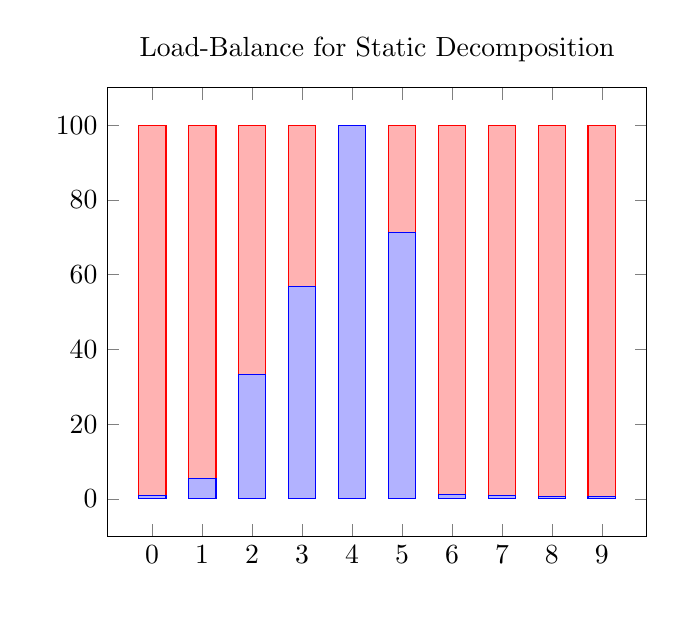
\begin{tikzpicture}
    \pgfplotstableread[col sep=comma, header=true]{
      process, working, waiting, communicating
      0,  0.91, 98.94, 0.15
      1,  5.42, 94.54, 0.03
      2, 33.25, 66.70, 0.05
      3, 56.85, 43.09, 0.06
      4, 99.92,  0.00, 0.08
      5, 71.39, 28.52, 0.09
      6,  1.21, 98.68, 0.11
      7,  0.78, 99.10, 0.12
      8,  0.68, 99.18, 0.14
      9,  0.60, 99.25, 0.15
    }\data

    \begin{axis}[
      ybar stacked
      , xtick={0, 1, ..., 9}
      , ymin=-10
      , ymax=110
      , ytick={0, 20, ..., 100}
      , title={Load-Balance for Static Decomposition}
      ]

      \addplot table[x=process, y=working] from \data;
      \addplot table[x=process, y=waiting] from \data;
      \addplot table[x=process, y=communicating] from \data;

    \end{axis}
  \end{tikzpicture}
  \caption{The load-balance for the Mandelbrot MPI static decomposition scheme,
    with 10 processes, where $N = 8000$, $\mathrm{maxiter} = 1000$. For each
    process, the percentage of time spent working is shown in blue, the
    percentage of time spent waiting in red, and the percentage of time spent
    communicating is shown in brown (however, this time is negligble and so is
    barely visible).}
  \label{fig:static-load-balance}
\end{figure}

\clearpage
\section{Master-Worker Scheme}
\label{sec:master-worker}

The Mandelbrot MPI master-worker scheme code,
\lstinline[style=ff]{src/mandelbrot_master_worker.f90}, can be
found in \autoref{sec:master-worker-code}.

% compare performance with static
For the case of a $8000 \cross 8000$ grid, and with
$\mathrm{chunksize} = 100000$, the Mandelbrot MPI master-worker scheme code
required \SI{18.548}{\second} to terminate, when run with 10 processes.
This is to say that it runs approximately 3.3 times faster than the MPI static
decomposition code, and 8.0 times faster than the serial code.
Furthermore, the load-balance is much more even across the worker processes with
very little time being spent idling, by any process.
The load-balance for the 9 worker processes is shown in
\autoref{fig:master-load-balance-100000}.
The master process is not included in the analysis of the load-balancing, since
it doesn't actually do any computational work, instead it simply orchestrates
the work done by the worker processes.
All the worker processes spend more than 99\% of their time working, which is
essentially ideal.
\begin{figure}[h]
  \centering
  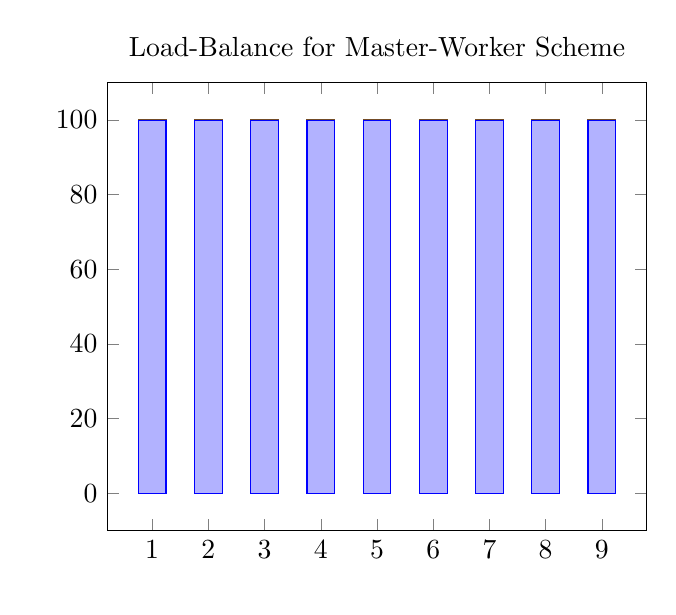
\begin{tikzpicture}
    \pgfplotstableread[col sep=comma, header=true]{
      process, working, waiting, communicating
      1, 99.80, 0.00, 0.20
      2, 99.83, 0.00, 0.17
      3, 99.81, 0.00, 0.19
      4, 99.80, 0.00, 0.20
      5, 99.80, 0.00, 0.20
      6, 99.80, 0.00, 0.20
      7, 99.78, 0.00, 0.22
      8, 99.82, 0.00, 0.18
      9, 99.79, 0.00, 0.21
    }\data

    \begin{axis}[
      ybar stacked
      , xtick={0, 1, ..., 9}
      , ymin=-10
      , ymax=110
      , ytick={0, 20, ..., 100}
      , title={Load-Balance for Master-Worker Scheme}
      ]

      \addplot table[x=process, y=working] from \data;
      \addplot table[x=process, y=waiting] from \data;
      \addplot table[x=process, y=communicating] from \data;

    \end{axis}
  \end{tikzpicture}
  \caption{The load-balance for the Mandelbrot MPI master-worker scheme,
    with 10 processes, where $N = 8000$, $\mathrm{maxiter} = 1000$, and
    $\mathrm{chunksize} = 100000$. For each worker process, the percentage of
    time spent working is shown in blue, the percentage of time spent waiting in
    red, and the percentage of time spent communicating is shown in brown;
    however, the time spent waiting and communicating is negligble and so both
    are barely visible.}
  \label{fig:master-load-balance-100000}
\end{figure}

% discuss how load balance varies with chunksize
The time taken for the Mandelbrot MPI master-worker scheme to terminate, for a
$8000 \cross 8000$ grid (that is, $64 \cross 10^{6}$ data points), for varying
chunk sizes is shown in \autoref{fig:scaling-chunksize}, when run with 10
processes (1 master process and 9 worker processes).
It can be seen that the elapsed time is effectively maximised across a range of
chunksizes which are neither too small nor too large compared to the total
number of data points, with elapsed times in the range of
\SIrange{18}{20}{\second}.

\begin{figure}[h]
  \centering
  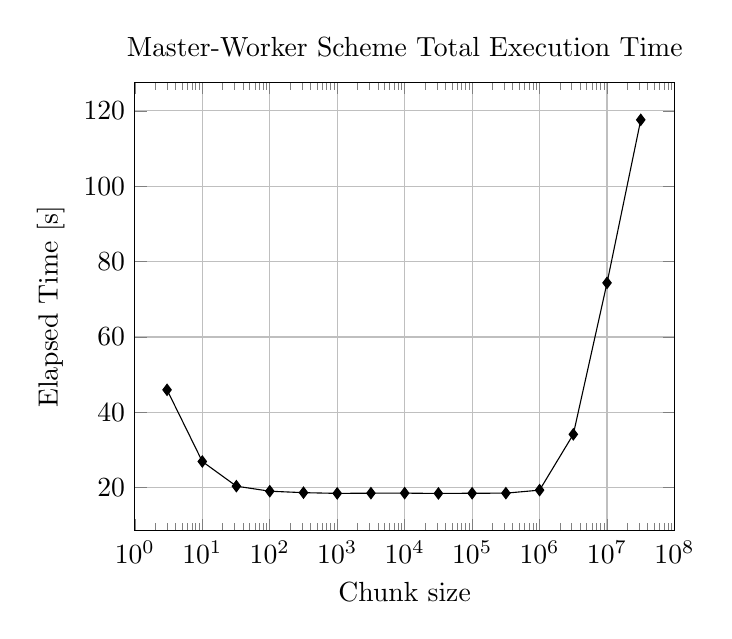
\begin{tikzpicture}
    \pgfplotstableread[col sep=comma, header=true]{
      chunksize, elapsedtime
      3, 45.985
      10, 26.966
      32, 20.422
      100, 19.087
      316, 18.700
      1000, 18.512
      3162, 18.560
      10000, 18.577
      31623, 18.492
      100000, 18.548
      316228, 18.569
      1000000, 19.368
      3162278, 34.179
      10000000, 74.364
      31622777, 117.62
    }\data

    \begin{axis}[
      use units
      , title = {Master-Worker Scheme Total Execution Time}
      , grid = major
      , xmode = log
      , log basis x = {10}
      , xlabel = {Chunk size}
      , ylabel = {Elapsed Time}
      , y unit = {s}
      , xmin = 1
      , xmax = 100000000
      ]

      \addplot [
      color = black
      , mark = diamond*
      ] table [x=chunksize, y=elapsedtime] \data;

    \end{axis}
  \end{tikzpicture}
  \caption{The total execution time for the Mandelbrot MPI master-worker scheme,
  with 10 processes, where $N=8000$, $\mathrm{maxiter}=1000$, for a range of
  chunk sizes, $\mathrm{chunksize} = 10^{k/2}$ for $k = 1, \dotsc, 15$. The MPI
  master-worker scheme, for a chunk size of $1$, failed to terminate within
  10 minutes and so was disregarded.}
  \label{fig:scaling-chunksize}
\end{figure}

However, for small chunk sizes, the elapsed time increases sharply (note that
the code failed to execute, for a chunksize of 1, in under 10 minutes).
This is to be expected as the amount of coordinating and MPI communication
overhead per chunk is constant, while the total number of chunks to work on is
increasing.
The total time can be estimated as the product of the average time per chunk and
the number of chunks, whence it is clear that as the chunk size decreasingly
tends to 1, the average time per chunk will tend to a constant, and so the total
time will increase
The load-balance for the 9 worker processes, for a chunksize of 10, is shown in
\autoref{fig:master-load-balance-10}.

\begin{figure}[h]
  \centering
  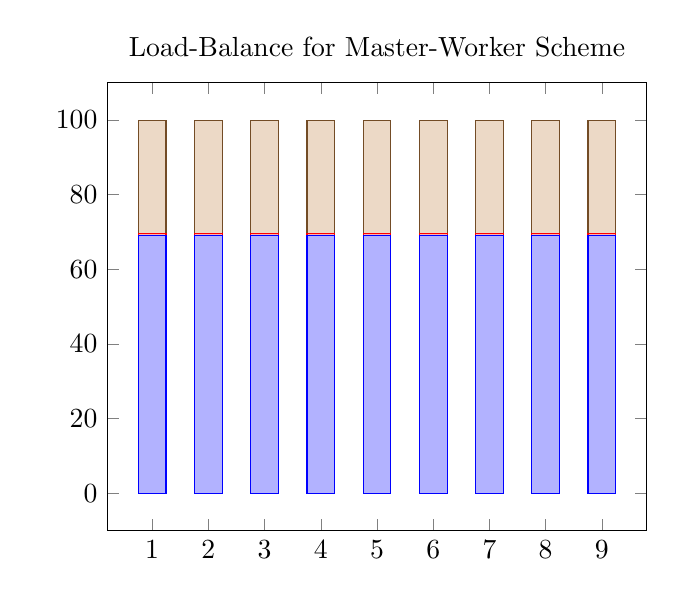
\begin{tikzpicture}
    \pgfplotstableread[col sep=comma, header=true]{
      process, working, waiting, communicating
      1, 68.99, 0.61, 30.18
      2, 69.00, 0.61, 30.18
      3, 69.02, 0.67, 30.09
      4, 68.95, 0.68, 30.14
      5, 69.01, 0.65, 30.12
      6, 69.02, 0.61, 30.15
      7, 68.98, 0.61, 30.15
      8, 69.02, 0.62, 30.14
      9, 68.99, 0.62, 30.17
    }\data

    \begin{axis}[
      ybar stacked
      , xtick={0, 1, ..., 9}
      , ymin=-10
      , ymax=110
      , ytick={0, 20, ..., 100}
      , title={Load-Balance for Master-Worker Scheme}
      ]

      \addplot table[x=process, y=working] from \data;
      \addplot table[x=process, y=waiting] from \data;
      \addplot table[x=process, y=communicating] from \data;

    \end{axis}
  \end{tikzpicture}
  \caption{The load-balance for the Mandelbrot MPI master-worker scheme,
    with 10 processes, where $N = 8000$, $\mathrm{maxiter} = 1000$, and
    $\mathrm{chunksize} = 10$. For each worker process, the percentage of
    time spent working is shown in blue, the percentage of time spent waiting in
    red, and the percentage of time spent communicating is shown in brown;
    however, the time spent waiting is negligble and so is barely visible.}
  \label{fig:master-load-balance-10}
\end{figure}

Furthermore, for large chunk sizes, the elapsed time also increases sharply,
which is to be expected.
As the chunk sizes become larger, the likelihood of a worker process being given
a chunk which requires more time to calculate than an average chunk increases.
Coupled with the fact that since there are fewer chunks to distribute among the
worker processes, the likelihood for some workers to be idling while other
workers finish up difficult chunks increases.
Hence, the load-balance becomes less ideal and so the efficiency of the
master-worker scheme decreases.
At extremely large chunk sizes, some processes may not even be assigned any
chunks to work on, which is obviously inefficient when it comes to
load-balancing.
The load-balance for the 9 worker processes, for a chunksize of 10000000, is
shown in \autoref{fig:master-load-balance-10000000}.

\begin{figure}[h]
  \centering
  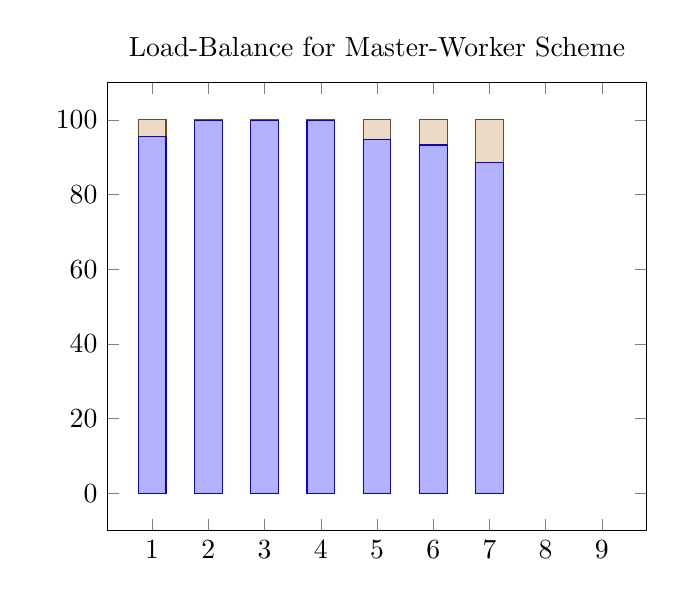
\begin{tikzpicture}
    \pgfplotstableread[col sep=comma, header=true]{
      process, working, waiting, communicating
      1, 95.54, 0.00, 4.45
      2, 99.81, 0.00, 0.19
      3, 99.94, 0.00, 0.06
      4, 99.93, 0.00, 0.07
      5, 94.72, 0.00, 5.27
      6, 93.26, 0.00, 6.73
      7, 88.58, 0.00, 11.41
      8,  0.00, 0.00, 0.00
      9,  0.00, 0.00, 0.00
    }\data

    \begin{axis}[
      ybar stacked
      , xtick={0, 1, ..., 9}
      , ymin=-10
      , ymax=110
      , ytick={0, 20, ..., 100}
      , title={Load-Balance for Master-Worker Scheme}
      ]

      \addplot table[x=process, y=working] from \data;
      \addplot table[x=process, y=waiting] from \data;
      \addplot table[x=process, y=communicating] from \data;

    \end{axis}
  \end{tikzpicture}
  \caption{The load-balance for the Mandelbrot MPI master-worker scheme,
    with 10 processes, where $N = 8000$, $\mathrm{maxiter} = 1000$, and
    $\mathrm{chunksize} = 10000000$. For each worker process, the percentage of
    time spent working is shown in blue, the percentage of time spent waiting in
    red, and the percentage of time spent communicating is shown in brown;
    however, the time spent waiting is negligble and so is barely visible.
    Note also that processes 8 and 9 are not present, this is due to them not
    being assigned any chunks at all, and thus terminated immediately.}
  \label{fig:master-load-balance-10000000}
\end{figure}

\clearpage
\section{Cyclic Decomposition}
\label{sec:cyclic}

The Mandelbrot MPI cyclic decomposition code,
\lstinline[style=ff]{src/mandelbrot_cyclic.f90}, can be found in
\autoref{sec:cyclic-code}.

% compare performance with static
For the case of a $8000 \cross 8000$ grid, the Mandelbrot MPI cyclic
decomposition code required \SI{17.393}{\second} to terminate, when run with 10
processes.
This is to say that it runs approximately 3.5 times faster than the MPI static
decomposition code, and 8.5 times faster than the serial code.
This is noticably faster than the MPI static decomposition code, while requiring
only minor modifications, in contrast with the significant additional complexity
of the MPI master-worker scheme code.

% discuss load imbalance
Furthermore, the load-balance is significantly more ideal than for the MPI
static decomposition code.
The load-balance for the 10 processes is shown in
\autoref{fig:cyclic-load-balance}.
All the processes spend more than 95\% of their time working, which is near
ideal.
\begin{figure}[h]
  \centering
  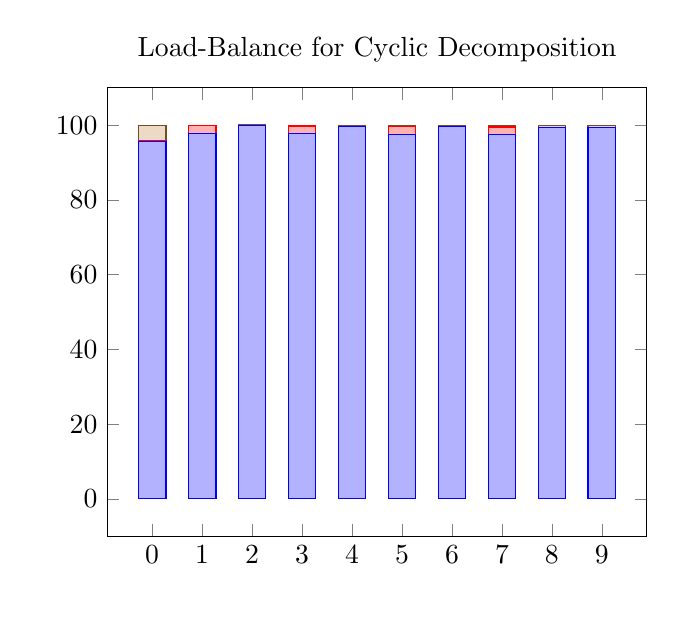
\begin{tikzpicture}
    \pgfplotstableread[col sep=comma, header=true]{
      process, working, waiting, communicating
      0, 95.76, 0.18, 4.06
      1, 97.86, 2.06, 0.08
      2, 99.86, 0.08, 0.13
      3, 97.74, 2.06, 0.20
      4, 99.67, 0.07, 0.26
      5, 97.61, 2.06, 0.33
      6, 99.55, 0.07, 0.38
      7, 97.49, 2.05, 0.46
      8, 99.41, 0.07, 0.51
      9, 99.30, 0.08, 0.62
    }\data

    \begin{axis}[
      ybar stacked
      , xtick={0, 1, ..., 9}
      , ymin=-10
      , ymax=110
      , ytick={0, 20, ..., 100}
      , title={Load-Balance for Cyclic Decomposition}
      ]

      \addplot table[x=process, y=working] from \data;
      \addplot table[x=process, y=waiting] from \data;
      \addplot table[x=process, y=communicating] from \data;

    \end{axis}
  \end{tikzpicture}
  \caption{The load-balance for the Mandelbrot MPI cyclic decomposition scheme,
    with 10 processes, where $N = 8000$, $\mathrm{maxiter} = 1000$. For each
    worker process, the percentage of time spent working is shown in blue, the
    percentage of time spent waiting in red, and the percentage of time spent
    communicating is shown in brown. It can be seen that the only process with
    non-negligble communication time is the root thread. This is due to the time
    spent re-ordering the cyclic data gathered at the root thread into the
    original sequential order being included in the time spent communicating for
    the root process. This was chosen since while cyclic decomposition may have
    benefits, untangling the returned data is a significant consideration.}
  \label{fig:cyclic-load-balance}
\end{figure}

The improvement of the cyclic decomposition over the static decomposition can be
explained by the nature of the Mandelbrot calculation.
Large contiguous regions of the grid may be trivially calculated, while other
regions may require far more iterations to calculate.
The difficulty of a given grid point, on average for certain regions, may be
similar to the difficulty of neighbouring grid points.
Hence, when a static decomposition is done, one process may be assigned a
trivial region while another is assigned a complex region.

However, under a cyclic decomposition, each process is assigned a number of
not-necessarily neighbouring grid points - preventing the accumulation of
trivial points in proximity by a single process.
Therefore, the average difficulty of each subset is likely to be much more
uniform than under a static decomposition, and thus the time spent working by
each process is also likely to be more uniform - leading to a more uniform
load-balance.
This is to say that the Mandelbrot calculation is more suited to a cyclic
decomposition than a static decomposition.

\clearpage
\appendix
\section{Appendix}
\label{sec:appendix}

\subsection{Serial}
\label{sec:serial-code}

\lstinputlisting[
language=Fortran
]{../src/mandelbrot.f90}

\newpage
\subsection{Static Decomposition}
\label{sec:static-code}

\lstinputlisting[
language=Fortran
]{../src/mandelbrot_static.f90}

\newpage
\subsection{Master Worker Scheme}
\label{sec:master-worker-code}

\lstinputlisting[
language=Fortran
]{../src/mandelbrot_master_worker.f90}

\newpage
\subsection{Cyclic Decomposition}
\label{sec:cyclic-code}

\lstinputlisting[
language=Fortran
]{../src/mandelbrot_cyclic.f90}


\end{document}